% !TEX root = ../diary-book.tex

\section{令和7年09月22日 ミューオンの到来数について）}
\label{sec:diary-20250922}

シャワー面の同定とミューオンの同定のどちらが効率的であるかということで、さまざまな位置に入射する一次粒子の影響を評価しようと試みた。サイトの中心を 1000 x 1000 m$^2$ の中で振ってみて、シャワー粒子（サイトに落とすエネルギーが 0.01 GeV 以上のもので、かつサイトが３つ以上ヒットする）とミューオンの数を調べた。

一次粒子のエネルギーが 100~TeV など高くなってくるとシャワー粒子の同定確率が高くなるが、低いときは単体のミューオン測定のほうが当然効率が上がってくる。
単純に地表面での観測をみるだけではミューオンのほうが効率がよいということになりそう。やっぱり地中の様子を見てみないことにはあまり強いことがいえなさそう。

\begin{figure}
  \centering
  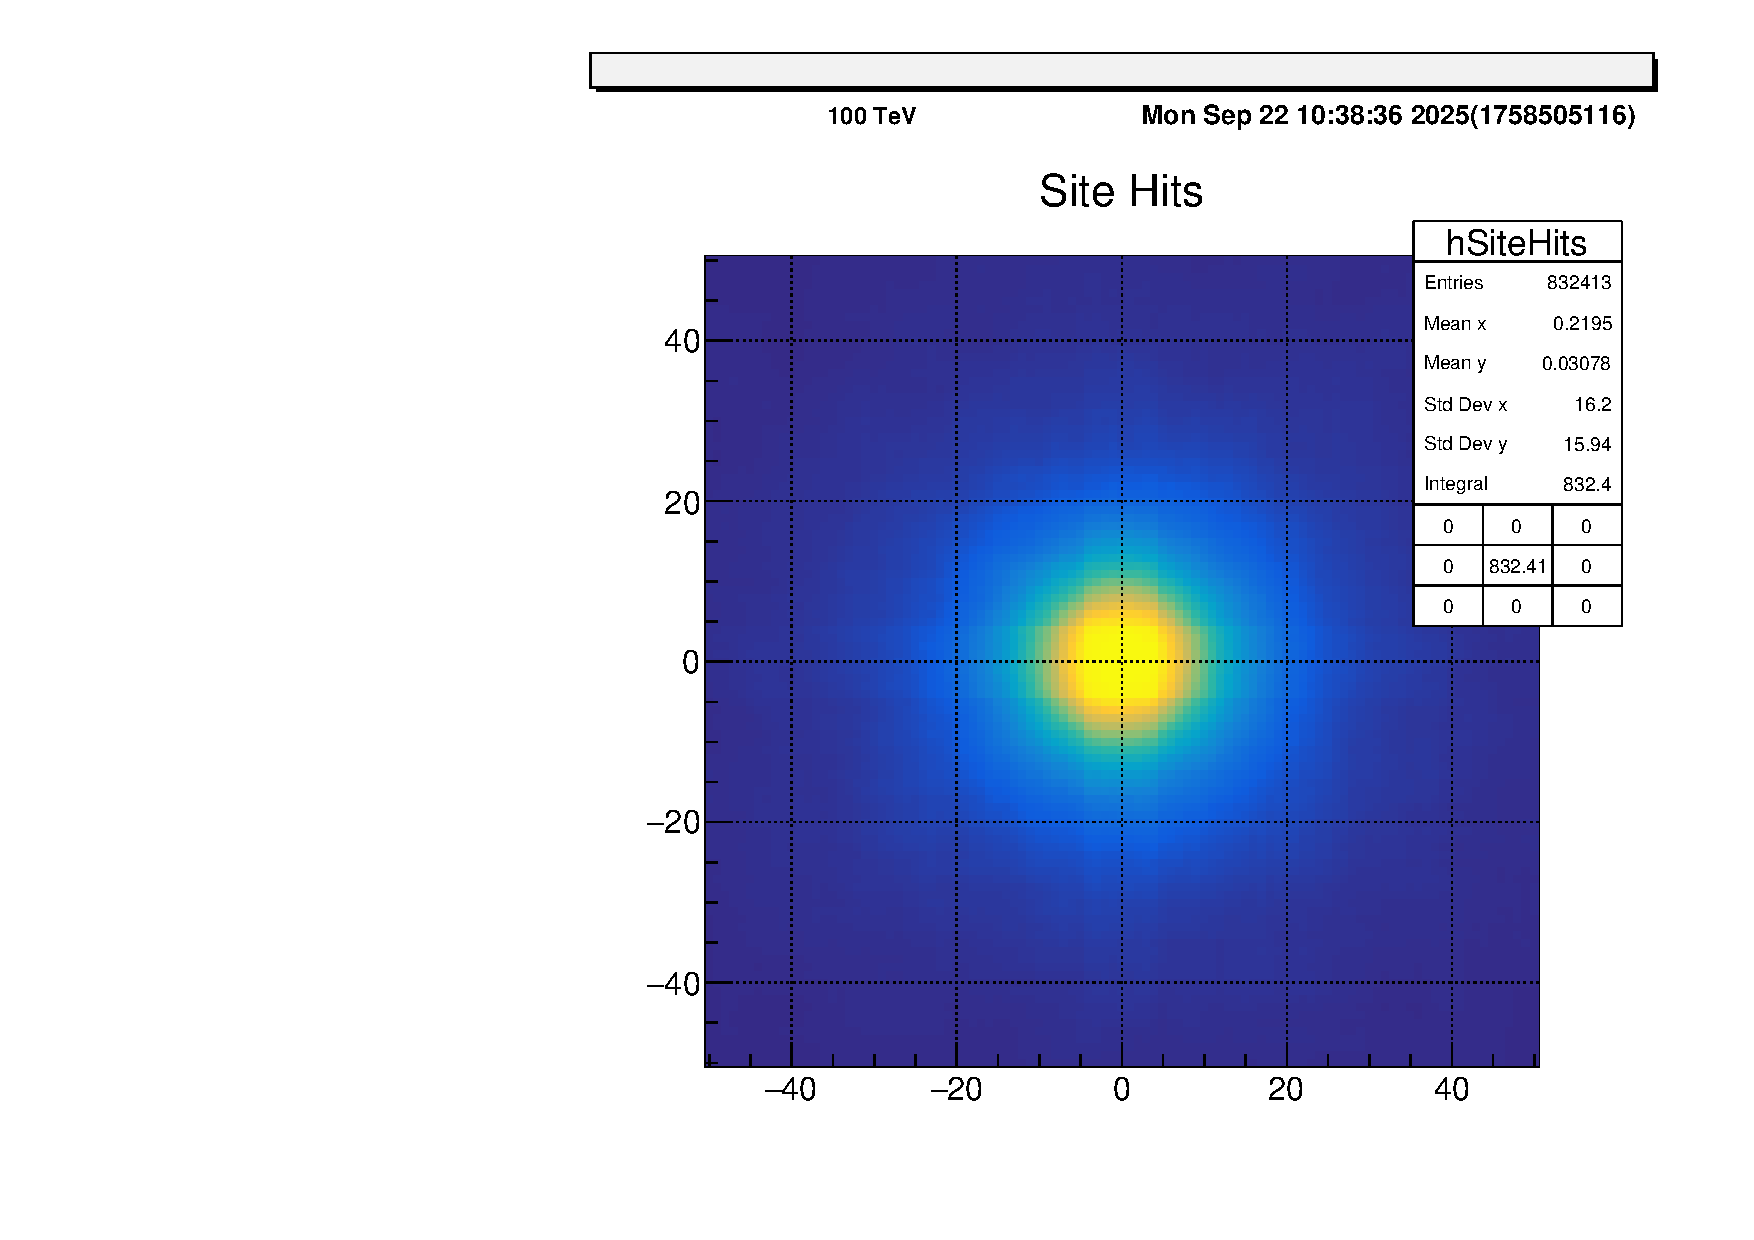
\includegraphics[width=0.6\textwidth]{figs/ata03/20250922/1758505116.pdf}
  \caption{Shower面同定数の２次元分布}
  \label{fig:shower_2d_dist}
\end{figure}
\begin{figure}
  \centering
  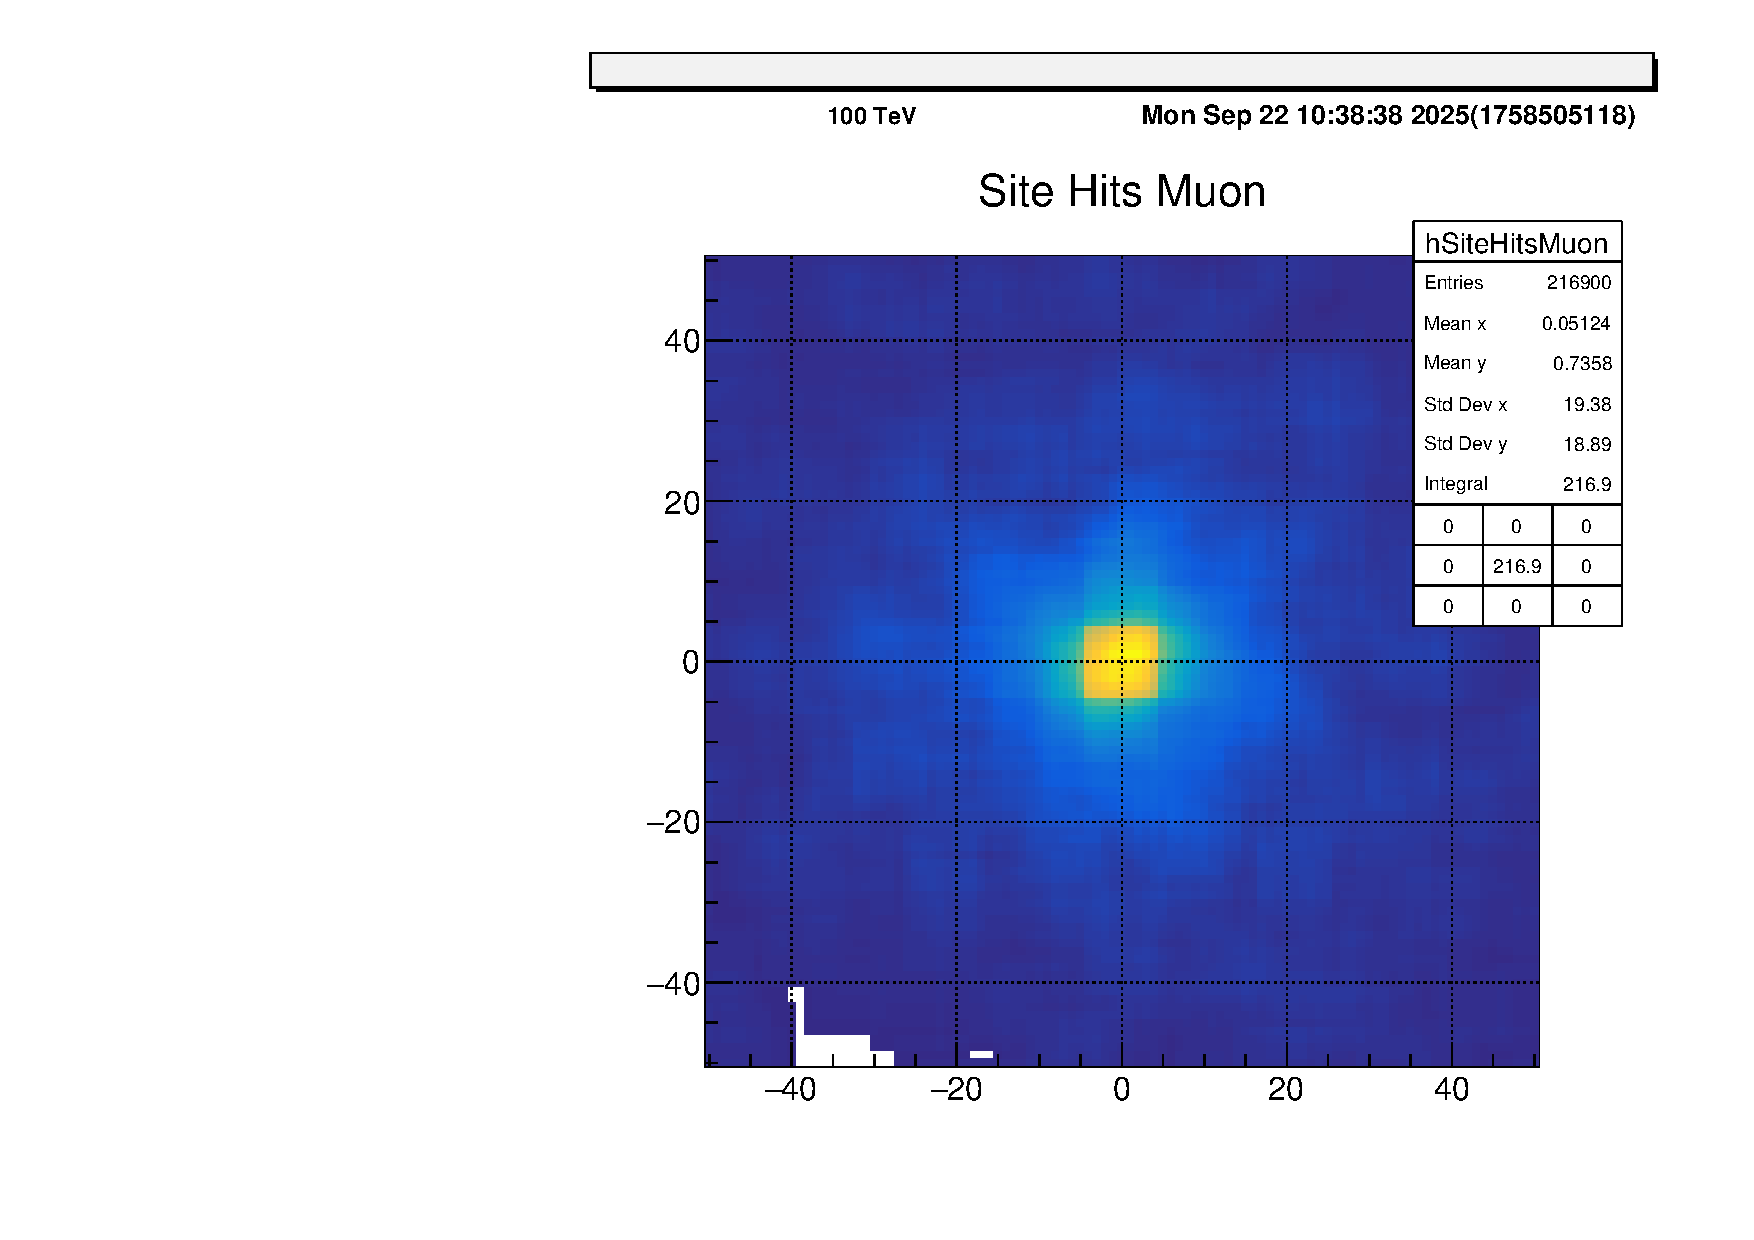
\includegraphics[width=0.6\textwidth]{figs/ata03/20250922/1758505118.pdf}
  \caption{ミューオン観測数の２次元分布}
  \label{fig:muon_2d_dist}
\end{figure}

\begin{figure}
  \centering
  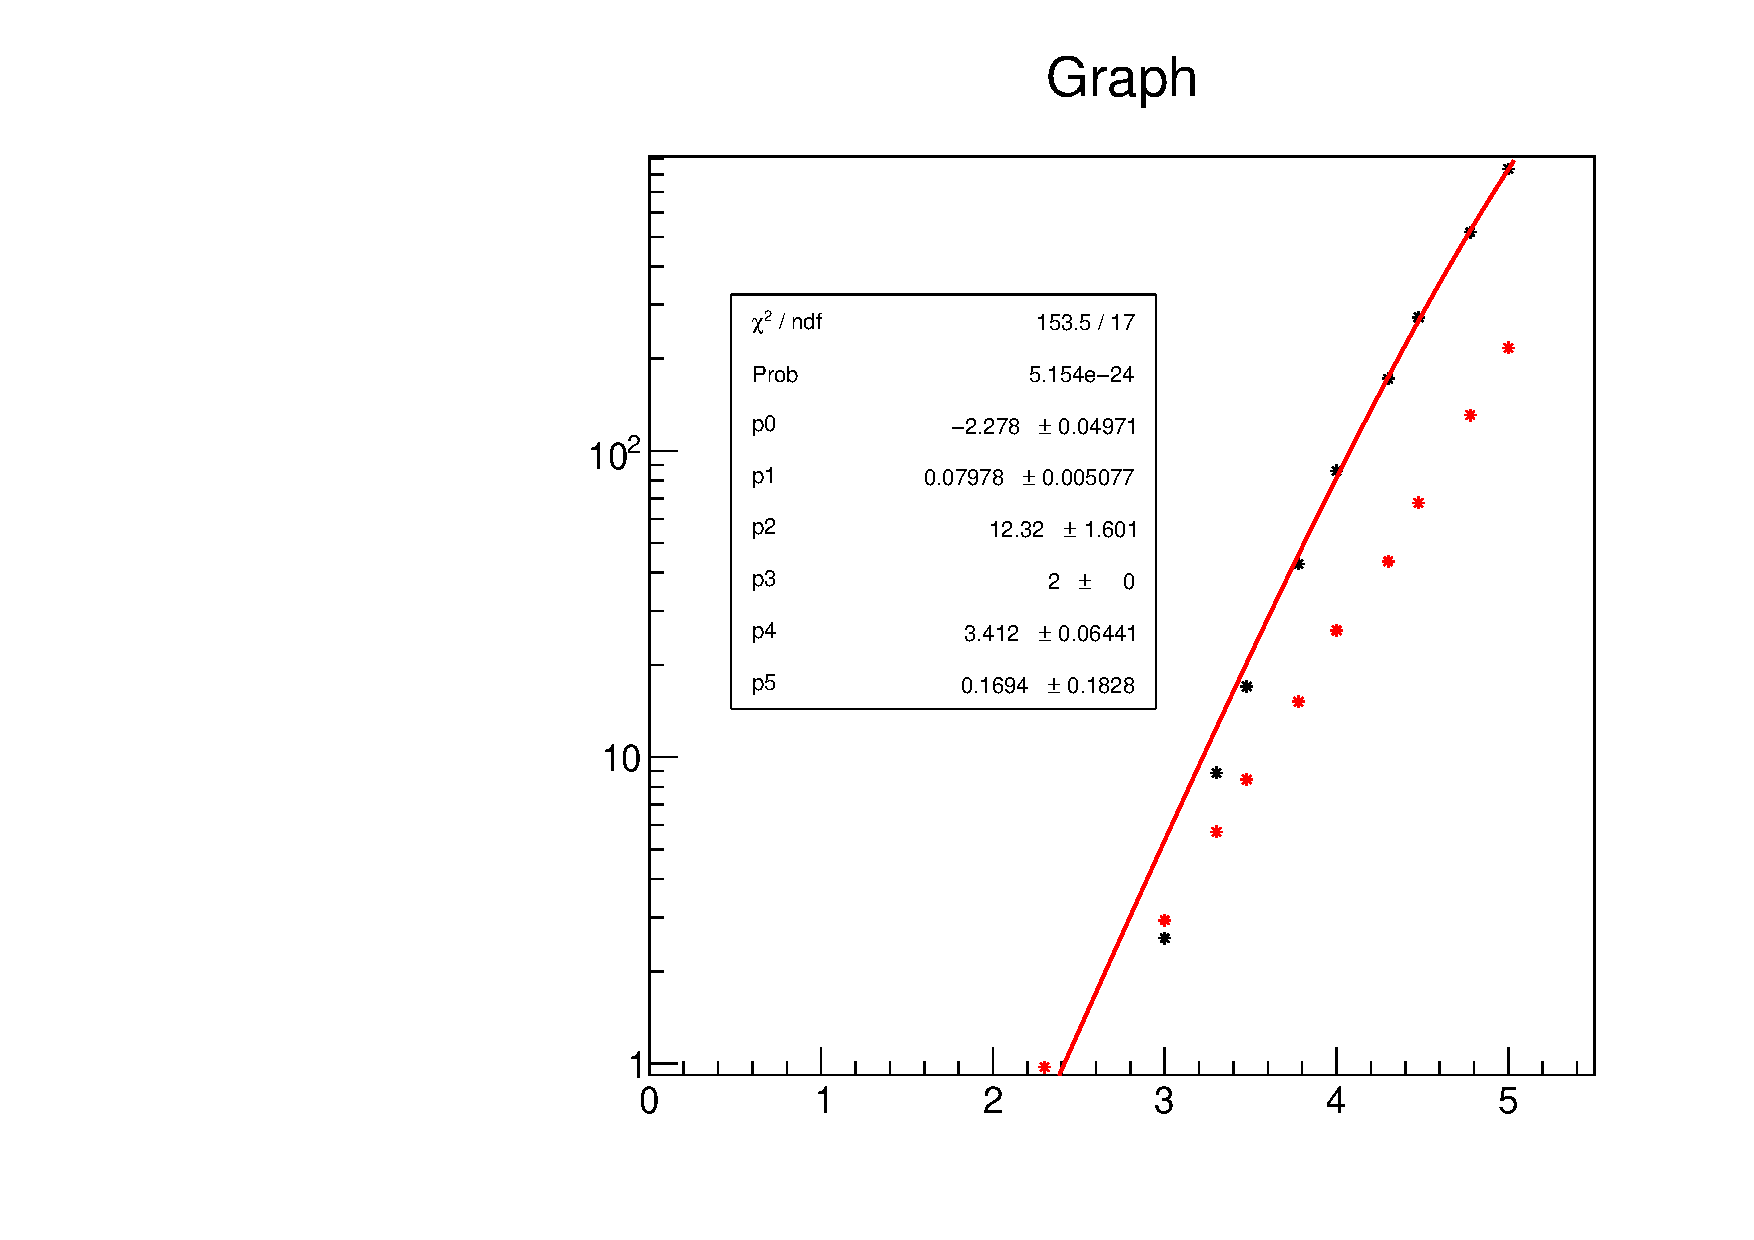
\includegraphics[width=0.6\textwidth]{figs/ata03/20250922/1758506590.pdf}
  \caption{シャワー面同定数とミューオンの観測数の比較}
  \label{fig:shower_muon_compare}
\end{figure}